\documentclass{article}
\usepackage[hyphens]{url}
\usepackage{xcolor}
\usepackage{fullpage}
\usepackage{graphicx}
\usepackage{epstopdf}
\usepackage{caption}
\usepackage{verbatim}
\usepackage{amssymb}
\usepackage{amsmath,amsthm}
\usepackage{amsfonts}
\usepackage{enumerate}
\usepackage{enumitem}
\usepackage{listings}
\usepackage{qtree}
\usepackage{tikz}
\usepackage{bm}
\usepackage{frame,color}
\usepackage{datetime}
\usepackage{etoolbox}
\usepackage{emerald}
\usepackage[T1]{fontenc}
\usepackage{bookmark}
\usepackage{multirow}
\usepackage{todonotes}
\usepackage[utf8]{inputenc}
\usepackage{glossaries}


\makeglossaries


\makeatletter
\patchcmd{\chapter}{\if@openright\cleardoublepage\else\clearpage\fi}{}{}{}
\makeatother
\definecolor{shadecolor}{rgb}{184,184,184}
\usetikzlibrary{calc,positioning}
\usetikzlibrary{arrows,automata}
\renewcommand{\familydefault}{\sfdefault}
\newglossaryentry{maths}
{
        name=mathematics,
            description={Mathematics is what mathematicians do}
}
 
\begin{document}
\sloppy

%%%%%%%%%%%%%%%%%%%%%%%%%%%%%%%%TITLE PAGE%%%%%%%%%%%%%%%%%%%%%%%%%%%%%%%%%%%%%%%%%%%%%%%%
\begin{figure}
    \begin{minipage}[H]{0.33\textwidth}
		\vspace{0.3cm}
		
\includegraphics[scale=0.8]{images/TUDelftLogo.eps}
	\end{minipage}
	\begin{minipage}[H]{0.33\textwidth}
		\begin{center}
			\ECFJD{Context Project\\Computer Games Group 8}
		\end{center}
		\begin{center}
			\includegraphics[scale=0.8]{images/Lg.eps}	
		
		\end{center}
	\end{minipage}
	\begin{minipage}[H]{0.425\textwidth}
			\begin{flushright}
				\small{Rob van Bekkum \qquad rvanbekkum\qquad 4210816}\\
				\small{Thijs Brands \qquad tlmbrands\qquad 4247132}\\
				\small{Soheil Jahanshahi \qquad sjahanshahi\qquad 4127617}\\
				\small{Aidan Mauricio \qquad amauricio\qquad 4195175}\\
				\small{Joost van Oorschot\qquad jjevanoorschot\qquad  4220471}\\
				\vspace{0.2cm}
				\small{\textbf{Date:} 15 May 2014}
			\end{flushright}
	\end{minipage} 
\end{figure}

\begin{minipage}[H]{\textwidth}
\vspace{0.3cm}
		\begin{center}
		  \vspace{0.3cm}
		  \Huge{\textbf{Emergent Architecture Design}}\\
		  \huge{Draft Version}
	      \vspace{0.3cm}	
   		  \vspace{0.7cm}	
		\end{center}
	\end{minipage}
%%%%%%%%%%%%%%%%%%%%%%%%%%%%%%%%%%%%%%%%%%%%%%%%%%%%%%%%%Document Starts Here%%%%%%%%%%%%%%%%%%%%%%%%%%%%%%%%%%%%%%%%%%%%%%%%%%%%%%%%%%%%%%%%%%%%%%%5
\tableofcontents
\newpage
	\section{Introduction}
	This document has been written with the goal of providing insight in the architecture design of our software solution. The architecture design will be subjected to change frequently due to the need for additional features or problems encountered with the current design. This document will be updated accordingly when these changes are made.
	 \subsection{Design goals}
	 \subsection{Loose Coupling}

We have divided our classes mostly over two categories: model and view. All classes that represent the game world or objects of the game world are part of the model. All classes that construct a way to view a part of the game world are part of the view category. One of our design goals was to keep coupling between these two categories as loose as possible. This way we can easily make changes to the game world our implement a new view without having to adjust a lot of classes.

\subsection{High cohesion}
It is very common that the strive for loose coupling is accompanied with the desire for high cohesion. We are no exception and want to keep cohesion as high as possible to ensure robustness and understandabillity of the code. This is why we always discuss  where in the software we should add new pieces of functionality, before actually implementing.

\subsection{Quality Code}

We strive for our code to have a certain level of quality. Writing good code makes it easier to expand the working prototype without having to fix emerging errors in the existing code. We want our code to approach the Exemplary Source Code Quality criteria as described in the Software Engineering Rubrics (2014).  This implies proper use of design patterns, very few design flaws and proper use of all software engineering principles. 

\subsection{Working Prototype}

We want to have a new working prototype at the end of every week. This will ensure that the features implemented in that week actually work when they are all integrated in one prototype. It also gives us the oppertunity to show our client early versions of our work on which we can get feedback. This feedback loop helps us make the product the client actually wants. The  working prototype also gives an indication of our current development stage and can give our client a feeling of progress.

	 \section{Software architecture views}
	 %\input{./sections/2.SoftwareArchitectureViews.tex}
	 \subsection{Subsystem decomposition} 
	 %(sub-systems and dependencies between them)

\begin{center}
	 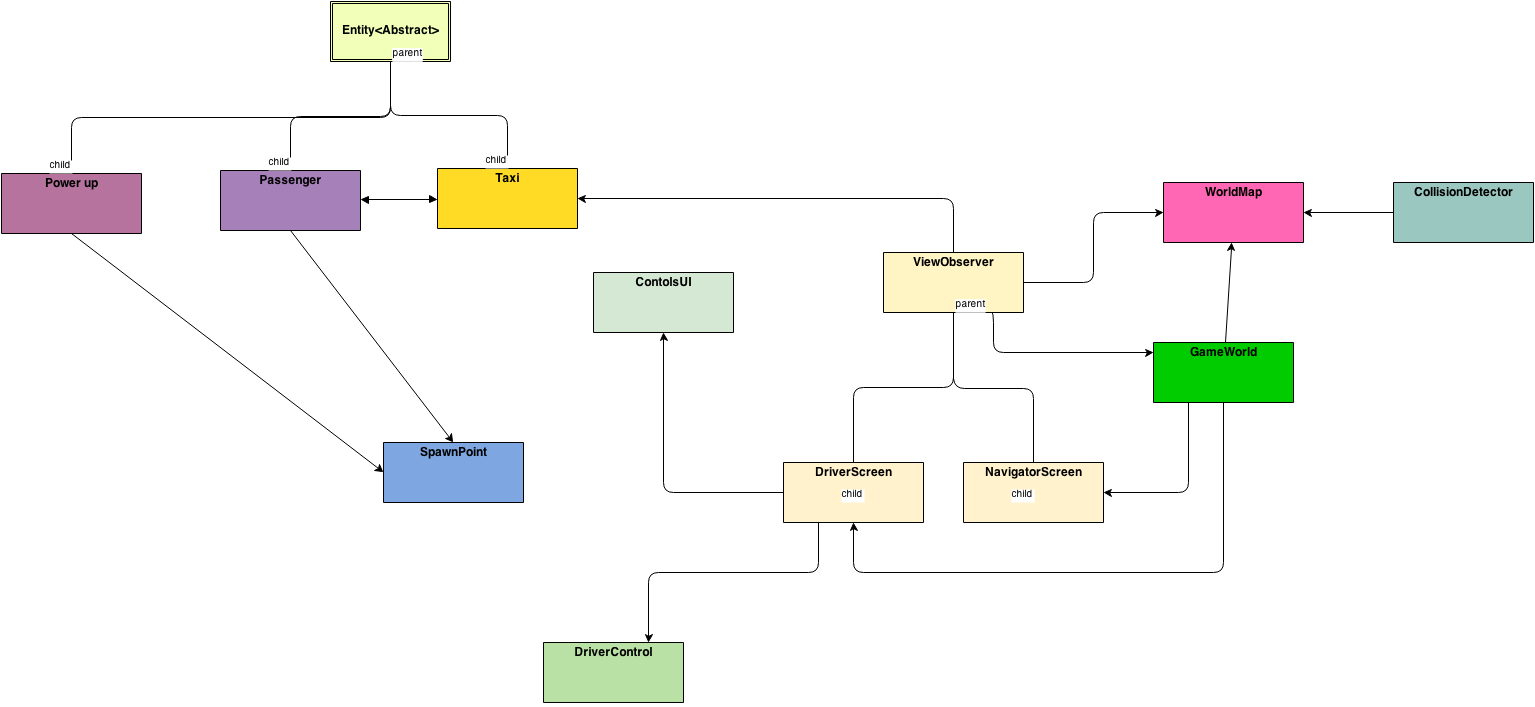
\includegraphics[width=180mm]{./images/UML4.png}

\end{center}


The architecture of the system is divided into subsystems. These subsystems are the Game Model, the Driver Interface, the Navigator Interface and the Network Interface. All subsytems will be explained in this section.

\begin{description}
	
\item[The Game Model] \hfill \\
The Game Model consists of the game world and all data related to the game. The actual game takes place in this subsystem. All other subsystems are interfaces that are used to alter the game model.

\item[The Driver Interface]  \hfill \\
This is one of the two interfaces that will be directly used by the players to interact with the Game Model. The Driver Interface enables the user to see the car and its direct surroundings. It also gives the user the means to controll the car (steering and acceleration). 

\item[The Navigator Interface]  \hfill \\
The second way for players to interact with the Game Model is the Navigator Interface. This interface gives the user an overview of the game world in the form of a map. This enables the user of this interface to (verbally) guide the user using the Driver Interface through the game world. The Navigator Interface can be used to interact with the Game Model through the activation of powerups, which will alter specific parts of the game world.

\item[The Network Interface]  \hfill \\
This interface is used to connect players with eachother. It is responsible for the connection of the two players within each team as well as the connection between all the teams. The Network Interface is also responsible for the concurrency between all Game Models.

\end{description}

	 \subsection{Hardware/software Mapping} 
	 
Taxi Trouble is a Real-Time Multi-player game where multiple users can join and interact with game instantaneously using their android devices. The game will start by main menu where User will choose his preferences. If User choses to have a role as `Taxi Driver' then Driver view UI is displayed otherwise User get a latter option as role of  `Navigator' and related UI will be displayed to the user. Since current subsystem design is experiencing its initial phase, there be more subsystem modification on the next sprints of the project.\\


\begin{center}
	 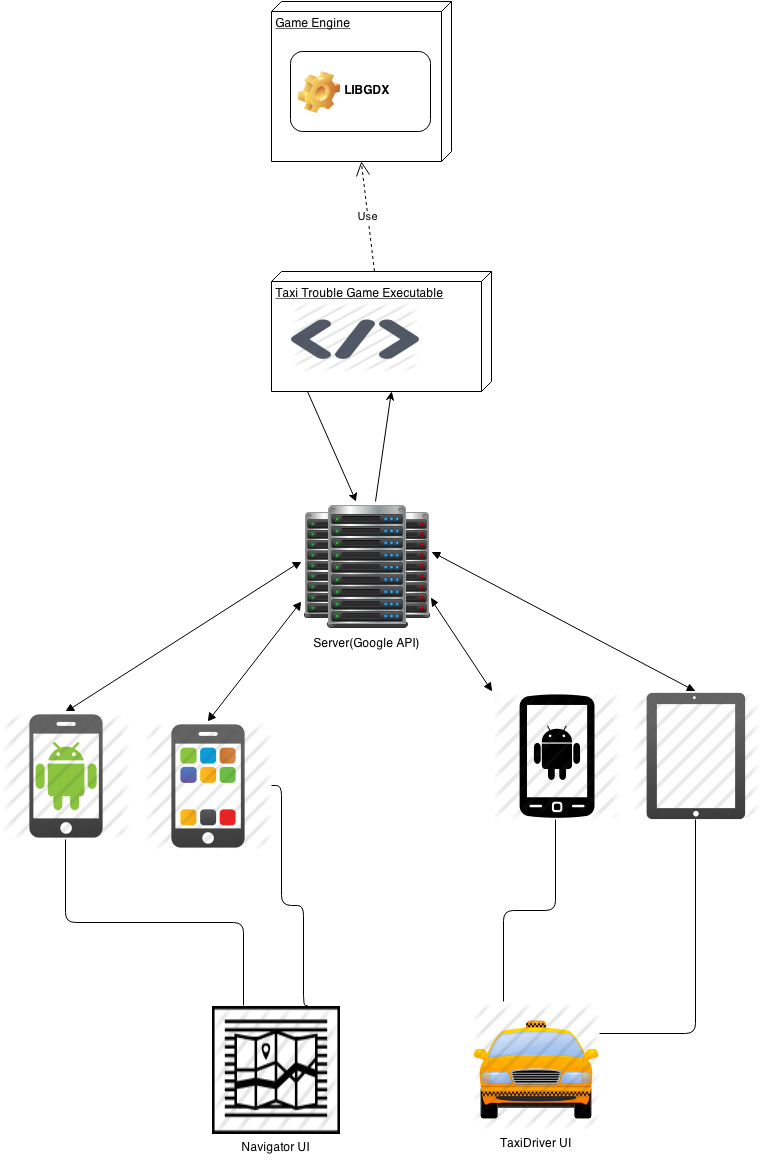
\includegraphics[width=130mm]{./images/hardsoft.png}
\end{center}
	\subsection{Persistent Data Management}
	The only persistent data in our game is the global leaderboard. This data is automatically handled by the Google Play Services API and stored on the Google Play Services Servers. 


	\subsection{Network Architecture}
	Our network architecture makes use of the Google Play Services (GPS)  API. This API sets up a peer to peer network between all clients playing the game. After establishing the peer to peer network, one of the clients is chosen to act as a server. The server will act as an authoritity, its state will be the "true" state of the game. Note that the client with the server role is still to be considered a functional client, although this client does have the advantage of playing directly on the server world. The table below lists all events that are sent over the network during normal gameplay.
\begin{center}
    \begin{tabular}{ | p{3cm} | l | l | p{7cm} |}
    \hline
    Event & Sent by &  Client-side & notes\\
	  &	        & prediction  & \\ \hline
    Car movement & Client &Yes  & Car movement is send by the client driving the car. \\ \hline
    Passenger pickup / dropoff / stealing  & Server & Yes & To prevent passengers being assigned to other taxis at the same time, only the server can send these events \\ \hline
   Powerup pickup & Server & Yes & To prevent power-ups being assigned to different teams at the same time, only the server can send this event. \\ \hline
 Powerup usage & Client & If needed  & We will implement client-side prediction and server reconciliation for powerups that are in need of this. \\ \hline
Create passenger / powerup & Server & No & New instances can only be spawned by the server, the clients should not try to predict this, as most spawning is random. \\ \hline
    \end{tabular}
\end{center}


If an event makes use of client-side prediction, the client (visually) simulates the event before receiving the event over the network. Upon receiving the actual event, the client can finalize and/or correct the simulated event.
	 \subsection{Concurrency} 
	 The only real type of concurrency we have to deal with is the concurrency of incomming messages. For sending critical game data, we use GPS's reliable messaging protocol which insures delivery, integrity and correct order of receival. For sending non-critical game data (ie. The location of a taxi),  we use GPS's unreliable messaging protocol. One might wonder what happens when two messages are received in such a way that two taxis are at the same location. The LibGDX game engine will handle this as a normal collide event and correct the location of the taxis accordingly.
	\section{Glossary}

	\begin{itemize}
		\item \textbf{Database} : A database is an organized collection of data.
		\item \textbf{Interface} : An interface is a shared boundary across which two separate components of a computer system exchange information. The exchange can be between software, computer hardware, peripheral devices, humans and combinations of these. 
		\item \textbf{Prototype} : A prototype is an early sample, model or release of a product built to test a concept or process or to act as a thing to be replicated or learned from.
		\item \textbf{Software Engineering Rubrics} is a document consisting of the different criteria for evaluation of our product. The document can be found on:  This implies proper use of design patterns, very few design flaws and proper use of all software engineering principles.
		\item \textbf{Subsystem Decomposition} :Also known as factoring, refers to the process by which a complex problem or system is broken down into parts that are easier to conceive, understand, program, and maintain.
		\item \textbf{libGDX}: libGDX is a game-development application framework written in the Java programming language with some C and C++ components for performance dependent code.
		\item \textbf{UI} :The user interface, in the industrial design field of human–machine interaction, is the space where interaction between humans and machines occurs.
		\item \textbf{ER} : an entity–relationship model (ER model) is a data model for describing the data or information aspects of a business domain or its process requirements, in an abstract way that lends itself to ultimately being implemented in a database such as a relational database.

		\section{References}
		
			\textbf{Software Engineering Rubrics} : \url{https://blackboard.tudelft.nl/bbcswebdav/pid-2235317-dt-content-rid-7624672_2/courses/30183-131404/SE\%20Rubrics.pdf}

			\textbf{Google Play Services} : \url{https://developers.google.com/games/services/common/concepts/realtimeMultiplayer}
 
		
	\end{itemize}


	\end{document}